%#! platex thesis.tex

%======================================================================
\chapter{実装}
\label{cha:imple}
本章では先行研究\cite{takahashi}で収集したデータについて説明し,本研究でのオンライン手書き医療用語認識手法の実装について説明する.
%----------------------------------------------------------------------
\section{データ収集}
\label{sec:collection}
本研究では,学習に使用したいデータがオープンソースで存在していないため,先行研究\cite{takahashi}において独自に収集しているデータを用いる.以下収集したデータの内容を説明する.

\subsection{医療用語コーパス}
\label{ssec:corpus}
過去の処方箋データから医療用語コーパスを作成している.コーパスとは,言語を分析するための基礎資料として書き言葉や話し言葉の資料を収集し,研究用の情報を付与したものである.本研究及び先行研究\cite{takahashi}では医療用語の手書き認識を行う.そこで \ref{sec:background}節で述べたPHCの過去の処方箋データからコーパスを作成し,それを機械学習の正解データとして用いている.8324名分の過去の処方箋データは,それぞれの欄が症状,薬名などに分けられる.先行研究\cite{takahashi}では薬名欄に頻出する単語(360語,英語)と医者からのアドバイス欄に頻出する単語(120語,バングラ語)を用いてコーパスを作成し,データ収集を行っている.データ提供者により手書きされた文字は正解データとともにデータベースに保存される.
%
%----------------------------------------------------------------------

\section{使用機器}
\label{sec:machine}
\textbf{図~\ref{equipments}}に使用機器を示す.機械学習には NVIDIA社の GeForce 1080 が1枚搭載された デスクトップ PC を用いた.\textbf{~\tablename~\ref{tab:spec}}に実装環境を示す.

\begin{figure}[tb]
 \begin{center}
  \includegraphics[keepaspectratio, scale=0.1]{img/equipments.png}
  \caption{使用機器}
  \label{equipments}
\end{center}
\end{figure}

\begin{table}[bt]
 \centering
 \caption{実装環境}
 \label{tab:spec}
 \begin{tabular}{ll}\Hline
  OS & \texttt{Ubuntu 16.04}\\
  GPU & \texttt{NVIDIA GeForce 1080}\\
  メモリ & \texttt{8GB}\\
  プロセッサ & \texttt{3.70GHz Intel Core i7-8000K}\\
 \Hline
 \end{tabular}
\end{table}

\section{学習モデル構造}
\textbf{図~\ref{layers}}に本研究で用いた学習モデルの構造を示す.文献\cite{zhang18:drawing}を参考に作成し,実装にはpythonのニューラルネットワークライブラリであるKeras\cite{keras}を用いている.本研究で用いるデータはデータ長が一定ではないため,データの後ろを$0$でパディングすることでデータ長最大の値である$260$に揃え,学習の入力とした.LSTM層の出力次元数は$300$に設定し,プールサイズの値の平均値をそれぞれ出力するプーリング層を配置した.その後パラメータの数を増やすために全結合層を配置した.なお,過学習を防ぐためプーリング層と全結合層の間にドロップアウト\cite{dropout}をそれぞれ$0.3$の割合で設定した.

\begin{figure}[tb]
 \centering
  \begin{tabular}{c}
    \begin{minipage}[b]{0.7\hsize}
     \centering
     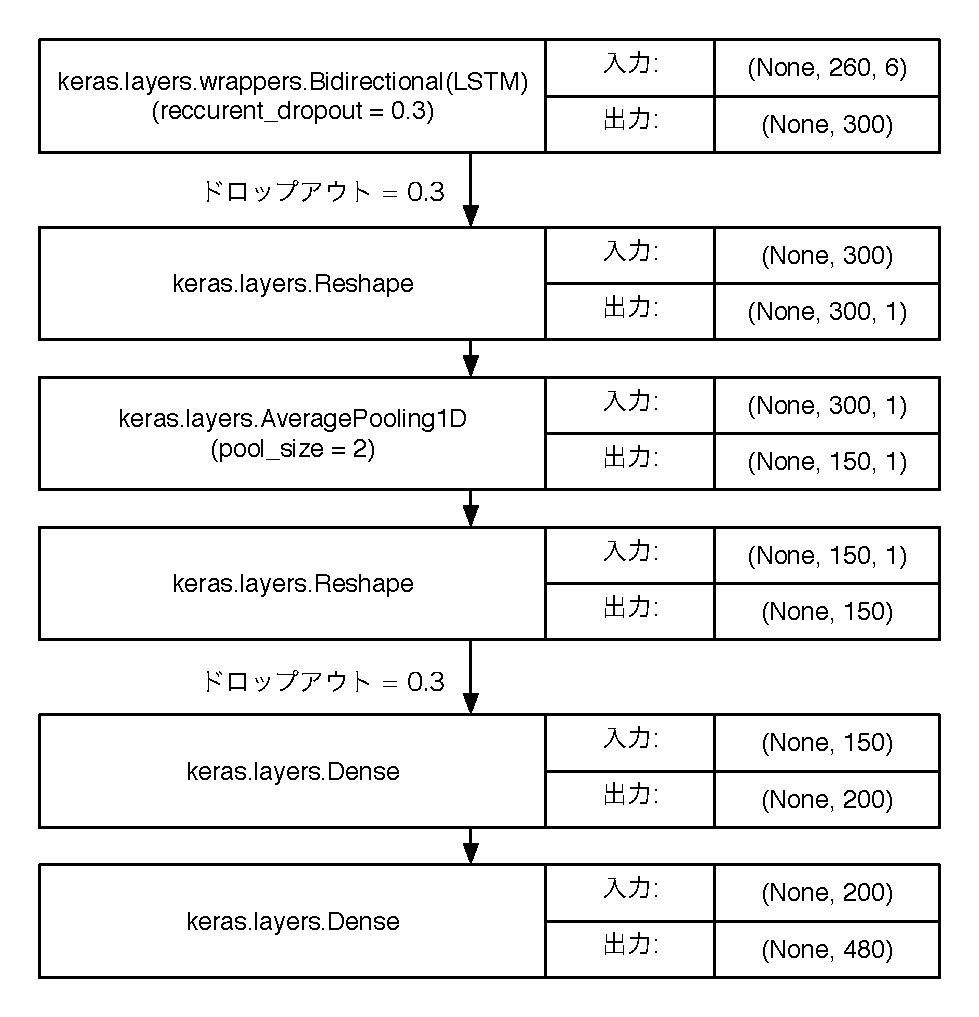
\includegraphics[keepaspectratio,scale=0.7]{img/layers.eps}\\
    \end{minipage}
  \end{tabular}
 \caption{層の構成}
 \label{layers}
\end{figure}

% 以下はRefTeX用
%%% Local Variables:
%%% mode: yatex
%%% TeX-master: "thesis"
%%% End:
